%!Mode:: "TeX:UTF-8"
\documentclass[a4paper,11pt,UTF8]{ctexart}

\usepackage{indentfirst} %缩进
\usepackage{xeCJK}    %使用系统字体
\usepackage{fancyhdr} %自定义页眉页脚
\pagestyle{plain}                   %不设置页眉页脚
\usepackage{amsmath, amsthm, amssymb, amsfonts} %数学公式
\usepackage[a4paper,left=3cm,right=3cm,top=3cm,bottom=3cm]{geometry}
%\usepackage[tmargin=1in,bmargin=1in,lmargin=1.25in,rmargin=1.25in]{geometry}.
\usepackage{booktabs} %插入表格
\usepackage[section]{placeins} %避免浮动
\usepackage{listings} %插入代码
\usepackage{ctex}     %中文宏包
\usepackage{bm}
\usepackage[svgnames, table]{xcolor} %彩色表格
\usepackage{algorithm}          %伪代码
\usepackage{algorithmicx}
\usepackage{algpseudocode}
\usepackage{algorithm,algpseudocode,float}
\usepackage{lipsum}
\usepackage{enumitem}           %调整列举环境
\usepackage{hyperref}
\hypersetup{
    colorlinks=true,
    linkcolor=blue,
    filecolor=blue,      
    urlcolor=blue,
    citecolor=cyan,
}
\usepackage{fontspec,xunicode}
\defaultfontfeatures{Mapping=tex-text} %如果没有它,会有一些 tex 特殊字符无法正常使用,比如连字符。

\usepackage{graphicx}
\graphicspath{{imgs/}}

%%%%%%%%%%%%%%%%%%%%%%%%%%%%%%%%%%%%%%%%%%%%%%%%%%%%%%%%%%%%%%%%
% 缩进及行间距
%%%%%%%%%%%%%%%%%%%%%%%%%%%%%%%%%%%%%%%%%%%%%%%%%%%%%%%%%%%%%%%%
\setlength{\parindent}{22pt} %重新定义缩进长度
\setlength{\baselineskip}{20pt}  %定义行间距
%\renewcommand{\baselinestretch}{1.1} %定义行间距

%%%%%%%%%%%%%%%%%%%%%%%%%%%%%%%%%%%%%%%%%%%%%%%%%%%%%%%%%%%%%%%%
% 列表设置
%%%%%%%%%%%%%%%%%%%%%%%%%%%%%%%%%%%%%%%%%%%%%%%%%%%%%%%%%%%%%%%%
\setenumerate{fullwidth,itemindent=\parindent,listparindent=\parindent,itemsep=0ex,partopsep=0pt,parsep=0ex}
\setenumerate[2]{label=\alph*),leftmargin=1.5em}  %二级item设置
\setitemize{itemindent=38pt,leftmargin=0pt,itemsep=-0.4ex,listparindent=26pt,partopsep=0pt,parsep=0.5ex,topsep=-0.25ex}
\setdescription{itemindent=38pt,leftmargin=0pt,itemsep=-0.4ex,listparindent=26pt,partopsep=0pt,parsep=0.5ex,topsep=-0.25ex}

%%%%%%%%%%%%%%%%%%%%%%%%%%%%%%%%%%%%%%%%%%%%%%%%%%%%%%%%%%%%%%%%
% 图的标题行间距设置
%%%%%%%%%%%%%%%%%%%%%%%%%%%%%%%%%%%%%%%%%%%%%%%%%%%%%%%%%%%%%%%%
\newcommand{\bottomcaption}{%
\setlength{\abovecaptionskip}{6pt}%
\setlength{\belowcaptionskip}{6pt}%
\caption}


%%%%%%%%%%%%%%%%%%%%%%%%%%%%%%%%%%%%%%%%%%%%%%%%%%%%%%%%%%%%%%%%
% 字体定义
%%%%%%%%%%%%%%%%%%%%%%%%%%%%%%%%%%%%%%%%%%%%%%%%%%%%%%%%%%%%%%%%
% \setmainfont{Times New Roman}  %默认英文字体.serif是有衬线字体sans serif无衬线字体
\setmonofont{Consolas}
\setCJKmainfont[ItalicFont={楷体}, BoldFont={黑体}]{宋体}%衬线字体 缺省中文字体为
\setCJKsansfont{黑体}
\punctstyle{hangmobanjiao}
%-----------------------xeCJK下设置中文字体------------------------------%
\setCJKfamilyfont{song}{SimSun}                             %宋体 song
\newcommand{\song}{\CJKfamily{song}}
\setCJKfamilyfont{fs}{FangSong}                      %仿宋  fs
\newcommand{\fs}{\CJKfamily{fs}}
\setCJKfamilyfont{ktgb}{KaiTi}                      %楷体2312 ktgb
\newcommand{\ktgb}{\CJKfamily{ktgb}}
\setCJKfamilyfont{yh}{Microsoft YaHei}                    %微软雅黑 yh
\newcommand{\yh}{\CJKfamily{yh}}
\setCJKfamilyfont{hei}{SimHei}                              %黑体  hei
\newcommand{\hei}{\CJKfamily{hei}}
\setCJKfamilyfont{hwxk}{STXingkai}                                %华文行楷  hwxk
\newcommand{\hwxk}{\CJKfamily{hwxk}}
%------------------------------设置字体大小------------------------%
\newcommand{\shiyanbaogao}{\fontsize{36pt}{\baselineskip}\selectfont}
\newcommand{\chuhao}{\fontsize{42pt}{\baselineskip}\selectfont}     %初号
\newcommand{\xiaochuhao}{\fontsize{36pt}{\baselineskip}\selectfont} %小初号
\newcommand{\yihao}{\fontsize{28pt}{\baselineskip}\selectfont}      %一号
\newcommand{\erhao}{\fontsize{21pt}{\baselineskip}\selectfont}      %二号
\newcommand{\xiaoerhao}{\fontsize{18pt}{\baselineskip}\selectfont}  %小二号
\newcommand{\sanhao}{\fontsize{15.75pt}{\baselineskip}\selectfont}  %三号
\newcommand{\sihao}{\fontsize{14pt}{\baselineskip}\selectfont}       %四号
\newcommand{\xiaosihao}{\fontsize{12pt}{\baselineskip}\selectfont}  %小四号
\newcommand{\wuhao}{\fontsize{10.5pt}{\baselineskip}\selectfont}    %五号
\newcommand{\xiaowuhao}{\fontsize{9pt}{\baselineskip}\selectfont}   %小五号
\newcommand{\liuhao}{\fontsize{7.875pt}{\baselineskip}\selectfont}  %六号
\newcommand{\qihao}{\fontsize{5.25pt}{\baselineskip}\selectfont}    %七号

%%%%%%%%%%%%%%%%%%%%%%%%%%%%%%%%%%%%%%%%%%%%%%%%%%%%%%%%%%%%%%%%
% 图题字体大小相同
%%%%%%%%%%%%%%%%%%%%%%%%%%%%%%%%%%%%%%%%%%%%%%%%%%%%%%%%%%%%%%%%
\usepackage{caption}
\captionsetup{font={footnotesize}}   % footnotesize = 9pt
\captionsetup[lstlisting]{font={footnotesize}}

%%%%%%%%%%%%%%%%%%%%%%%%%%%%%%%%%%%%%%%%%%%%%%%%%%%%%%%%%%%%%%%%
% 重定义枚举编号为 1),2)...
%%%%%%%%%%%%%%%%%%%%%%%%%%%%%%%%%%%%%%%%%%%%%%%%%%%%%%%%%%%%%%%%
\renewcommand{\labelenumi}{\theenumi)}


%%%%%%%%%%%%%%%%%%%%%%%%%%%%%%%%%%%%%%%%%%%%%%%%%%%%%%%%%%%%%%%%
% 重定义section标题
%%%%%%%%%%%%%%%%%%%%%%%%%%%%%%%%%%%%%%%%%%%%%%%%%%%%%%%%%%%%%%%%
\CTEXsetup[format={\sihao\CJKfamily{zhhei}\zihao{4}},number={\chinese{section}},name={,、~},aftername={},indent={0pt},beforeskip={6pt},afterskip={6pt},format+={\flushleft}]{section}
\CTEXsetup[format={\Large\bfseries\CJKfamily{zhkai}\zihao{4}},name={(,)},number={\chinese{subsection}},aftername={},indent={22pt},beforeskip={14pt},afterskip={2pt}]{subsection}
\CTEXsetup[number={\chinese{section}},name={附录, ~~ }]{appendix}



%%%%%%%%%%%%%%%%%%%%%%%%%%%%%%%%%%%%%%%%%%%%%%%%%%%%%%%%%%%%%%%%
% 标题名称中文化
%%%%%%%%%%%%%%%%%%%%%%%%%%%%%%%%%%%%%%%%%%%%%%%%%%%%%%%%%%%%%%%%
\renewcommand\figurename{\hei 图}
\renewcommand\tablename{\hei 表}
\renewcommand\lstlistingname{\hei 代码}
\renewcommand{\algorithmicrequire}{\textbf{输入:}}
\renewcommand{\algorithmicensure}{\textbf{输出:}}
\newtheorem{define}{定义}

%%%%%%%%%%%%%%%%%%%%%%%%%%%%%%%%%%%%%%%%%%%%%%%%%%%%%%%%%%%%%%%%
% 代码设置
%%%%%%%%%%%%%%%%%%%%%%%%%%%%%%%%%%%%%%%%%%%%%%%%%%%%%%%%%%%%%%%%
\lstset{frame=tb,
  language=Python,
  aboveskip=3mm,
  belowskip=3mm,
  showstringspaces=false,
  columns=flexible,
  basicstyle={\small\ttfamily},
  numbers=none,
  numberstyle=\tiny\color{gray},
  keywordstyle=\color{blue},
  commentstyle=\color{dkgreen},
  stringstyle=\color{mauve},
  breaklines=true,
  breakatwhitespace=true,
  tabsize=3
}

%%%%%%%%%%%%%%%%%%%%%%%%%%%%%%%%%%%%%%%%%%%%%%%%%%%%%%%%%%%%%%%%
% 伪代码分页
%%%%%%%%%%%%%%%%%%%%%%%%%%%%%%%%%%%%%%%%%%%%%%%%%%%%%%%%%%%%%%%%
\makeatletter
\renewcommand{\ALG@name}{算法}
\newenvironment{breakablealgorithm}
  {% \begin{breakablealgorithm}
   \begin{center}
     \refstepcounter{algorithm}% New algorithm
     \hrule height.8pt depth0pt \kern2pt% \@fs@pre for \@fs@ruled
     \renewcommand{\caption}[2][\relax]{% Make a new \caption
       {\raggedright\textbf{\ALG@name~\thealgorithm} ##2\par}%
       \ifx\relax##1\relax % #1 is \relax
         \addcontentsline{loa}{algorithm}{\protect\numberline{\thealgorithm}##2}%
       \else % #1 is not \relax
         \addcontentsline{loa}{algorithm}{\protect\numberline{\thealgorithm}##1}%
       \fi
       \kern2pt\hrule\kern2pt
     }
  }{% \end{breakablealgorithm}
     \kern2pt\hrule\relax% \@fs@post for \@fs@ruled
   \end{center}
  }
\makeatother



\begin{document}
\xiaosihao\song

\begin{titlepage}
\center{\yihao{\hei{机器学习课程实验报告}}}
\vspace{6cm}
\center{\erhao{\ktgb{PCA模型}}}
\vspace{4cm}

\begin{center}
\begin{large}
\begin{tabular}{rc}
\xiaoerhao{\hei{学\qquad 号}}& \hspace{1.7cm}\xiaoerhao{\hei{1180301007\hspace{1.7cm}}} \\
\cline{2-2}\\
\xiaoerhao{\hei{姓\qquad 名}}& \xiaoerhao{\hei{赵锦涛}}\\
\cline{2-2}\\
\xiaoerhao{\hei{实验时间}}& \xiaoerhao{\hei{2020年10月}}\\
\cline{2-2}
\end{tabular}
\end{large}
\end{center}
\vfill \hfill
\end{titlepage}
\clearpage


\setlength{\parskip}{6pt}  %定义段间距

\section{实验目的:}
实现一个PCA模型,能够对给定数据进行降维(即找到其中的主成分)。
\section{实验要求:}
(1)首先人工生成一些数据(如三维数据),让它们主要分布在低维空间中,如首先让某个维度的方差远小于其它唯独,然后对这些数据旋转。生成这些数据后,用你的PCA方法进行主成分提取。 \\
(2)找一个人脸数据(小点样本量),用你实现PCA方法对该数据降维,找出一些主成分,然后用这些主成分对每一副人脸图像进行重建,比较一些它们与原图像有多大差别(用信噪比衡量)。 \\


\section{实验环境:}
Python 3.8, Windows 10
\section{实验原理:}
PCA算法有两种形式:最大方差形式和最小误差形式。给定一组数据${x_{n}}$,样本集合的均值表达为:
$$ \bar x = \frac{1}{N} \sum_{n=1}^{N}x_{n}$$
投影数据的方差为
$$
\frac{1}{N} \sum_{n=1}^{N}\{\boldsymbol{u}_{1}^{T} \boldsymbol{x}_{n}-\boldsymbol{u}_{1}^{T} \overline{\boldsymbol{x}}\}^{2}=\boldsymbol{u}_{1}^{T} \boldsymbol{S} \boldsymbol{u}_{1}
$$
考虑M维投影空间的一般情形,那么最大化投影数据方差的最优线性投影由数据协方差矩阵S的M个特征 向量$u_{1},...,u_{m}$定义,对应于M个最大的特征值$\lambda_{1}, ..., \lambda_{m}$. \\
对于最小误差形式,不失⼀般性,M维线性⼦空间可以⽤前M个基向量表⽰,因此我们可以⽤下式来近似每个数据点$x_{n}$
$$
J=\frac{1}{N} \sum_{n=1}^{N}\|\boldsymbol{x}_{n}-\tilde{\boldsymbol{x}}_{n}\|^{2}
$$
进一步,我们可以得到失真度量的对应的值为:
$$ J = \sum_{i = M + 1}^{D} \lambda_{i}$$
于是,我们可以通过将这些特征向量选择成D-M个最小的特征值对应的特征向量,来得到J的最小值,因此定义了主子空间的特征向量是对应于M个最大特征值的特征向量。 \\
PCA算法可分为以下几个步骤:
\begin{itemize}
  \item Step 1: 求平均值以及做normalization
  \item Step 2: 求协方差矩阵(Covariance Matrix),在实验中使用的是散度矩阵(Scatter Matrix)
  \item Step 3: 求协方差矩阵的特征根和特征向量
  \item Step 4: 选择主要成分
  \item Step 5: 转化得到降维的数据
\end{itemize}
\section{代码实现}
本次实验共有3个文件,其名称和作用分别为:
\begin{itemize}
  \item \emph{datagen.py} \quad 生成训练数据
  \item \emph{pca.py} \quad PCA算法实现
  \item \emph{cv\_test.py} \quad 使用PCA算法对图片进行降维
\end{itemize}
其中PCA算法的实现为
\begin{lstlisting}[caption={PCA},captionpos=b]
def pca(x, k):
    x_mean = np.mean(x)
    x_norm = x - x_mean
    s_Cov = np.dot(np.transpose(x_norm), x_norm)
    eig_val, eig_vec = np.linalg.eig(s_Cov)
    index = np.argsort(-eig_val)
    index = index[0:k]
    pc = eig_vec[:, index]
    new_data = np.dot(np.dot(x - x_mean, pc), pc.T) + x_mean
    return new_data, pc, x_mean
\end{lstlisting}

\section{实验结果与分析}
使用PCA对满足二维高斯分布的点进行降维,结果如图所示:
\begin{figure}[H]
  \centering
  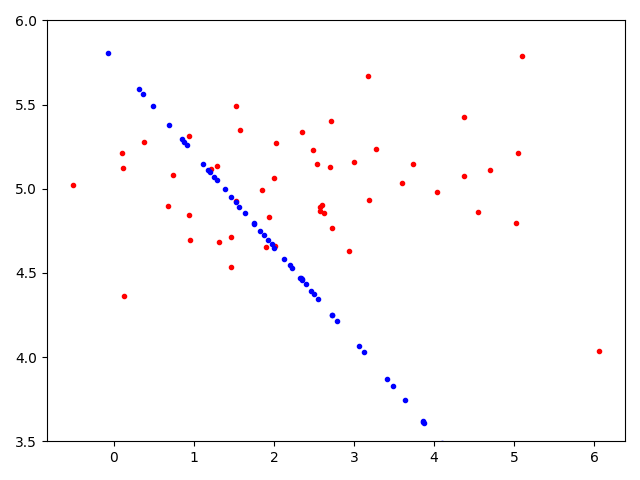
\includegraphics[width=0.6\textwidth]{2D.png}
  \bottomcaption{二维数据降维}
\end{figure}
对三维数据提取主成分,结果如图所示:
\begin{figure}[H]
  \centering
  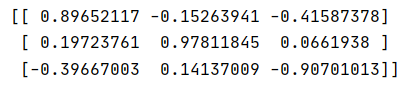
\includegraphics[width=0.6\textwidth]{3D_PC.png}
  \bottomcaption{三维数据主成分}
\end{figure}
使用PCA对图像进行降维有(原图像为$250 \times 250$,转换为灰度图像降到80维):
\begin{figure}[H]
  \centering
  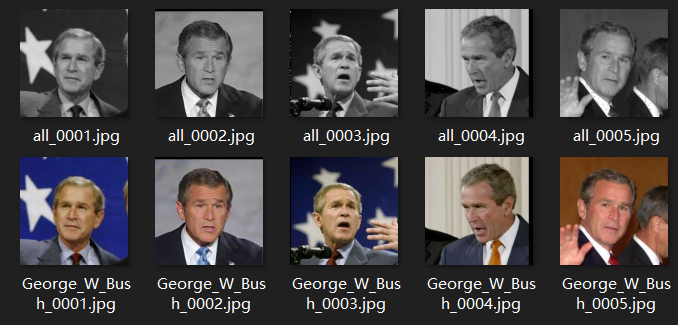
\includegraphics[width=0.6\textwidth]{cmp1.png}
  \bottomcaption{降维图片第一部分}
\end{figure}
\begin{figure}[H]
  \centering
  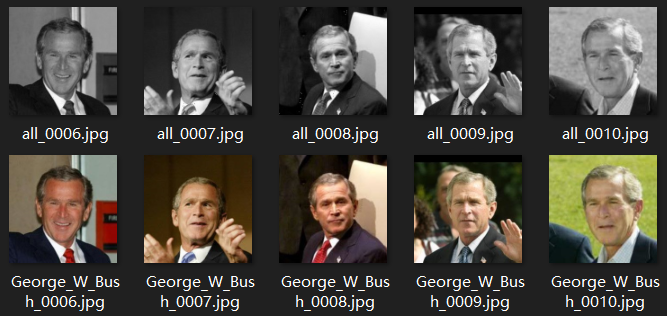
\includegraphics[width=0.6\textwidth]{cmp2.png}
  \bottomcaption{降维图片第二部分}
\end{figure}
计算得到的信噪比为:
\begin{figure}[H]
  \centering
  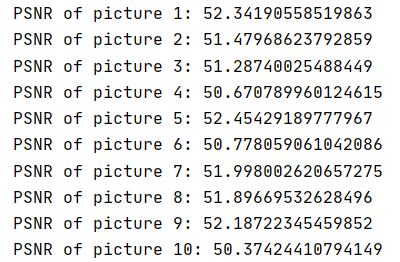
\includegraphics[width=0.6\textwidth]{PSNR.png}
  \bottomcaption{信噪比}
\end{figure}
从实验结果可以看出,PCA算法可以很好地保留原有数据的主要成分。
\begin{thebibliography}{99} 
\bibitem{ref1}Bishop C M. Pattern recognition and machine learning[M]. springer, 2006.
\end{thebibliography}



\end{document}
